\documentclass{article}
\usepackage[utf8]{inputenc}
\usepackage{tikz}
\usetikzlibrary{arrows.meta}

\begin{document}

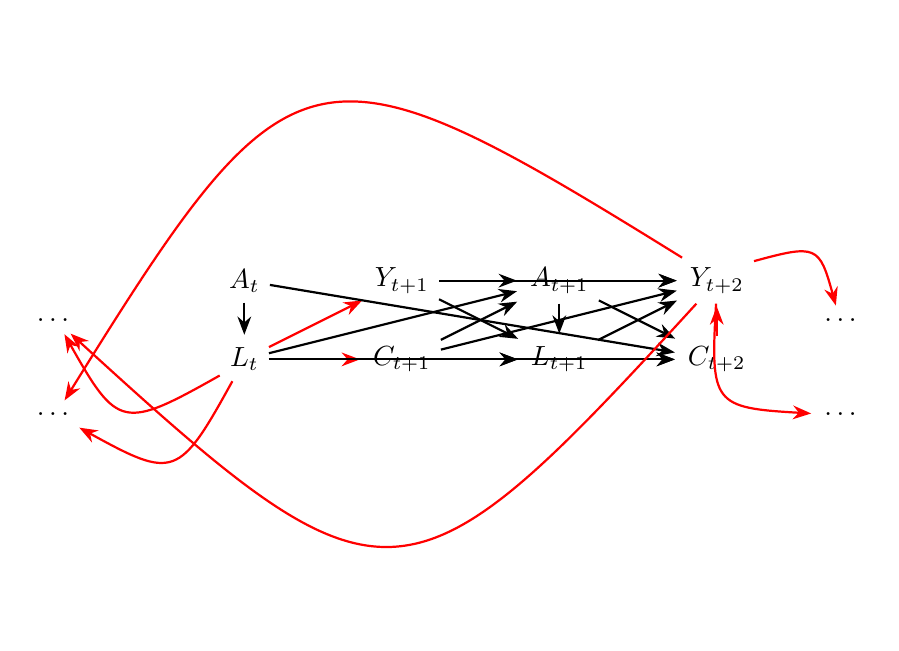
\begin{tikzpicture}[->,>=Stealth,shorten >=1pt,auto,node distance=3cm,
                thick,main node/.style={circle,draw,font=\sffamily\Large\bfseries}]

    \node[fill=none] (dots1) at (-4,0) {\ldots};
    \node[fill=none] (dots2) at (-4,-1.2) {\ldots};

    \node[fill=none] (A_t) at (-1.6, 0.5) {$A_{t}$};
    \node[fill=none] (Y_t) at (-1.6, -0.5) {$L_{t}$};
    \node[fill=none] (Y_tp1) at (0.4, 0.5) {$Y_{t+1}$};
    \node[fill=none] (A_tp1) at (0.4, -0.5) {$C_{t+1}$};
    \node[fill=none] (Y_tp2) at (2.4, 0.5) {$A_{t+1}$};
    \node[fill=none] (Y_tp3) at (2.4, -0.5) {$L_{t+1}$};
    \node[fill=none] (Y_tp4) at (4.4, 0.5) {$Y_{t+2}$};
    \node[fill=none] (C_tp4) at (4.4, -0.5) {$C_{t+2}$};
    \node[fill=none] (dots3) at (6,0) {\ldots};
    \node[fill=none] (dots4) at (6,-1.2) {\ldots};

    \path[every node/.style={font=\sffamily\small}]
        % Arrows between nodes
        (A_t) edge node {} (Y_t)
        (Y_t) edge [red] node {} (Y_tp1)
        (Y_t) edge [red] node {} (A_tp1)
        (Y_t) edge node {} (Y_tp2)
        (Y_t) edge node {} (Y_tp3)
        (Y_t) edge node {} (C_tp4)
        (A_t) edge node {} (C_tp4)
        (Y_tp1) edge node {} (Y_tp2)
        (Y_tp1) edge node {} (Y_tp3)
        (Y_tp1) edge node {} (Y_tp4)
        (A_tp1) edge node {} (Y_tp2)
        (A_tp1) edge node {} (Y_tp3)
        (A_tp1) edge node {} (Y_tp4)
        (Y_tp2) edge node {} (Y_tp3)
        (Y_tp2) edge node {} (Y_tp4)
        (Y_tp2) edge node {} (C_tp4)
        (Y_tp3) edge node {} (Y_tp4)
        (Y_tp3) edge node {} (C_tp4)
        (C_tp4) edge [red] node {} (Y_tp4)
        (Y_tp4) edge [bend right=45, looseness=1.75, red] node {} (dots4)
        (Y_tp4) edge [bend left=45, looseness=1.75, red] node {} (dots3)
        (Y_tp4) edge [bend right=45, looseness=1.75, red] node {} (dots2)
        (Y_tp4) edge [bend left=45, looseness=1.75, red] node {} (dots1)
        (Y_t) edge [bend left=45, looseness=1.75, red] node {} (dots2)
        (Y_t) edge [bend left=45, looseness=1.75, red] node {} (dots1);

\end{tikzpicture}

\end{document}